\documentclass[12pt, french]{article}

\usepackage{fancyhdr, fancybox, lastpage,mhchem}
\usepackage[most]{tcolorbox}
\usepackage[a4paper, margin={0.3in, .75in}]{geometry}
\usepackage{wrapfig}
\pagestyle{fancy}
\renewcommand\headrulewidth{1pt}
\renewcommand\footrulewidth{1pt}
\fancyhf{}
\rhead{ \em{Zakaria Haouzan}}
\lhead[C]{\em{2ème année baccalauréat Sciences Physiques}}
\chead[C]{}
\rfoot[C]{}
\lfoot[R]{}
\cfoot[]{\em{Page \thepage / \pageref{LastPage}}}


\newtcolorbox{Box2}[2][
enhanced, 
    breakable,
]{
                lower separated=false,
                colback=white,
colframe=white!20!black,fonttitle=\bfseries,
colbacktitle=white!30!gray,
coltitle=black,
enhanced,
attach boxed title to top left={yshift=-0.1in,xshift=0.15in},
title=#2,#1}


\begin{document}
\begin{center}
   \shadowbox {\bf{Transformations spontanées dans les piles}
 }

\end{center}

\vspace{-0.2cm}
%%_________________________Exercice ! :"_________________________Exercice
   \begin{Box2}{Exercice 1 :}
On réalise une pile en utilisant le matériel et les produits suivants :

\begin{itemize}
	\item un bêcher contenant le volume $V_1 = 20 mL$ d’une solution aqueuse de nitrate d’argent $Ag^+_{(aq)}$+$NO^-_{3(aq)}$ de concentration molaire $ C_1 =1,0.10^- mol/L$.

	\item un bêcher contenant le volume $V_2=20 mL$ d’une solution aqueuse de nitrate de cuivre $Cu^{2+}_{(aq)} $+$ 2NO^-_{3(aq)}$ de concentration molaire  $C =5,0.10^{-2} mol/L$
	\item  un fil de cuivre et  un fil d’argent ;
	\item un pont salin contenant une solution aqueuse saturée de nitrate de potassium $K^+_{(aq)} + NO^-_{3(aq)}$
	\item $1F=96500 C/mol$ 
	\item Constante d’équilibre associée à l’équation \ce{$2Ag^+_{(aq)}$ + $Cu_{(s)}$ <=> $2Ag_{(s)}$ + $Cu^{2+}_{(aq)}$ } est $K = 2,2.10^{15}$
\end{itemize}

On relie les électrodes de la pile à un conducteur ohmique en série avec un ampèremètre, et on
observe le passage d’un courant électrique dans le circuit extérieur de la pile.
\begin{enumerate}
	\item  Calculer la valeur du quotient de la réaction $Qr,i$
dans l’état initial du système chimique. En déduire
le sens spontané de l’évolution de ce système.

\item  On fait fonctionner la pile pendant une longue durée jusqu’ ce qu’il s’épuise. Déterminer la valeur
de la quantité d’électricité qui traverse le conducteur ohmique depuis le début de fonctionnement de la
pile jusqu'à son épuisement, sachant que le réactif limitant est l’ion
$Ag^+$ .


\end{enumerate}
   \end{Box2}


%%_________________________Exercice !2 :"_________________________Exercice
\begin{Box2}{Exercice 2 :}
%\begin{wrapfigure}{r}{0.22\textwidth}
  %\begin{center}
	  %\vspace{-0.6cm}
	%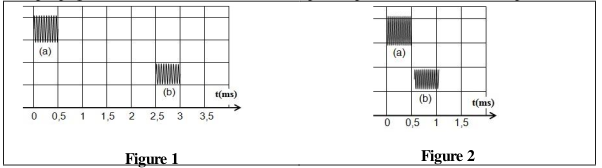
\includegraphics[width=0.22\textwidth]{./img/Ex2.png}
  %\end{center}
%\end{wrapfigure}

Le but de cette partie est l’étude d'une transformation spontanée dans une pile.
On considère la pile Zinc/Argent. Cette pile est constituée des éléments suivants:
\begin{itemize}
	\item Un bécher contenant une solution aqueuse de nitrate d'argent $Ag^+_{(aq)} + NO^-_{3(aq)}$ de volume $V_1$
		et de concentration molaire $C_1 = 2,0.10^{-1} mol/L$.


\item  Un bécher contenant une solution aqueuse de nitrate de zinc $Zn^{2+}_{(aq)} + 2NO^-_{3(aq)}$ de volume $V_2$ et
	de concentration molaire $C_2 = 2,0.10^{-2} mol/L$

\item  Un fil d'argent $Ag_{(s)}$

\item Une plaque mince du zinc $Zn_{(s)}$

\item  Un pont salin.

\item Constante d’équilibre associée à l’équation \ce{$2Ag^+_{(aq)}$ + $Zn_{(s)}$ <=>[1][2] $2Ag_{(s)}$ + $Zn^{2+}_{(aq)}$ } est $K = 10^{52}$

\end{itemize}

On branche, en série aux bornes de la pile, un ampèremètre et un conducteur ohmique. Le circuit est
alors traversé par un courant électrique.

\begin{enumerate}
	\item Déterminer la valeur du quotient de réaction $Q_{r,i}$
, du système chimique à l'état initial .

\item  Déduire, en justifiant votre réponse, le sens d'évolution spontané du système chimique lors du
fonctionnement de la pile. 
\item . On laisse la pile fonctionner pendant une durée très longue jusqu'à ce qu'elle s'épuise.
Déterminer la valeur de la quantité d’électricité maximale Qmax
, qui a traversé le conducteur ohmique
du début de fonctionnement de la pile jusqu'à ce qu'elle s'épuise sachant que l’avancement maximale
est $x_{max} = 5.10^{-3}mol$
\end{enumerate}

\end{Box2}

\vspace{-0.8cm}
\begin{center}
   \Large{ \em{Exercices Supplémentaires}}
\end{center}

\vspace{-0.8cm}

%%_________________________Exercice ! 3:"_________________________Exercice
\begin{Box2}{Exercice 3 : }
\begin{wrapfigure}{r}{0.4\textwidth}
  \begin{center}
	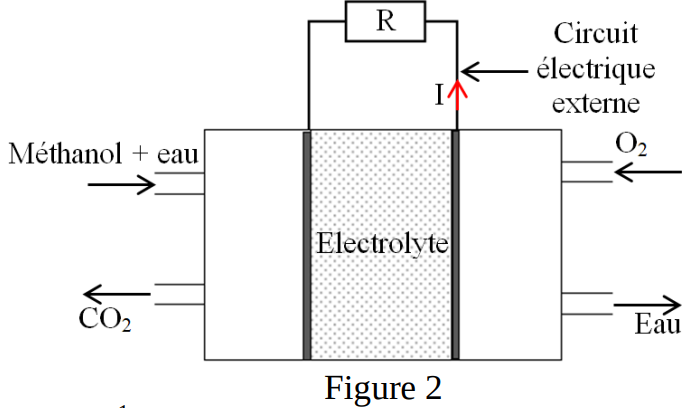
\includegraphics[width=0.4\textwidth]{./ex02.png}
  \end{center}
\end{wrapfigure}

Cette pile est constituée de deux
compartiments séparés par un
électrolyte acide, jouant le rôle
d’un pont ionique et de deux
électrodes A et B.
La pile est alimentée, au cours du
fonctionnement, par du méthanol
liquide et du dioxygène gazeux.
(Figure 2)

\textbf{Données :}
\begin{itemize}
	\item Masse volumique du méthanol liquide : $\rho$=$ 0,78 g.cm^{-3}$.
	\item Masse molaire du méthanol : $M = 32 g.mol^{-1}$ 
	\item Les couples intervenants dans la transformation: $(O_{2(g)}/H_2O_{(l)})$ et $(CO_{2(g)}/CH_3OH_{(l)})$
\end{itemize}

Au cours du fonctionnement de la pile, il se produit au voisinage de l’une des  électrodes une transformation modélisée par l’équation suivante : 
$$\ce{CH_3OH_{(l)} + H_2O_{(l)} ->  CO_{2(g)} + a.H^+ + b.e^- } $$

\begin{enumerate}
	\item Déterminer les coefficients a et b.
	\item Préciser au voisinage de quelle électrode A ou B, se produit cette réaction ?
	\item Ecrire l’équation modélisant la réaction ayant lieu au voisinage de l’autre
électrode. Nommer les deux électrodes A et B.
\item La pile alimente le circuit extérieur par un courant d’intensité $I = 45 mA$
supposée constante durant $\Delta{t} = 1 h 30 min$. Trouver la valeur du volume $V$
de méthanol consommé au cours de la durée $\Delta{t}$ de fonctionnement.
\end{enumerate}


\end{Box2}

%%_________________________Exercice 4 : _________________________Exercice
\begin{Box2}{Exercice 4 : }
   % \begin{wrapfigure}[12]{r}{0.5\textwidth}
  %\begin{center}
	  %\vspace{-0.6cm}
	%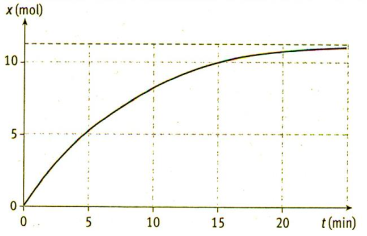
\includegraphics[width=0.5\textwidth]{./img/ex4.png}
  %\end{center}
%\end{wrapfigure}

	On réalise la pile constituée des couples $(Ni^{2+}_{(aq)}/Ni_(s))$ et $(Zn^{2+}_{(aq)}/Zn_{(s)})$ en immergeant L’électrode de Nickel dans une solution de sulfate de Nickel $(Ni^{2+}_{(aq)} + SO^{2-}_{4(aq)})$ de 
volume $V = 150 mL$ et de concentration molaire initiale $[Ni^{2+}_{(aq)}]_i=10^{-2} mol/L$.


L’électrode de Zinc dans une solution de sulfate de Zinc $(Zn^{2+}_{(aq)} +SO^{2-}_{4(aq)})$
de volume $V = 150 mL$ et de concentration molaire initiale ,On relie les deux compartiments par un pont ionique. La constante d’équilibre associée à l’équation de la réaction suivante est $K=10^{18}$ : \\\ce{$Ni^{2+}_{(aq)}$ + $Zn_{(s)}$ <=>[1][2] $Ni_{(s)}$ + $Zn^{2+}_{(aq)}$ } est $K = 10^{52}$

	1. Préciser, en calculant le quotient de réaction $Q_{r,i}$ à l’état initial, le sens spontané
d’évolution du système constituant la pile.

2. Donner le schéma conventionnel de la pile étudiée.

3. Au cours du fonctionnement de la pile, le circuit extérieur est traversé par un
courant d’intensité $I = 0,1 A$. Trouver la durée maximale $\Delta{t}_{max}$ de fonctionnement de la pile en fonction de : $[Zn^{2+}_{(aq)}]_i$ , V, F et I .Calculer $\Delta{t}_{max}$


\end{Box2}



%\vspace{-0.6cm}
%%%_________________________Exercice 5 : _________________________Exercice
%\begin{Box2}{Exercice 4 : }
   %% \begin{wrapfigure}[14]{r}{0.5\textwidth}
  %%\begin{center}
	  %%\vspace{-0.6cm}
	%%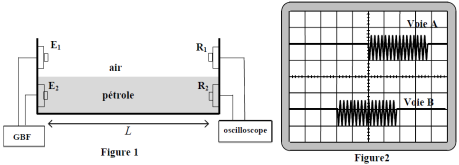
\includegraphics[width=0.5\textwidth]{./img/ex5.png}
  %%\end{center}
%%\end{wrapfigure}

%4

%\end{Box2}

%\begin{Box2}{Exercice 5 : }

%44
%\end{Box2}


%\begin{Box2}{Exercice 6 : }


	%\end{Box2}


%\begin{Box2}{Exercice 7 : }
%\end{Box2}
\end{document}
